%
% 2_beispiel.tex -- Wellengleichung tatsächlich lösen mit der Methode
%
% (c) 2025 Roman Cvijanovic & Nicola Dall'Acqua, Hochschule Rapperswil
%
% !TEX root = ../../buch.tex
% !TEX encoding = UTF-8
%

\section{Rechenbeispiel}\label{neuronal:section:rechenbeispiel}
\kopfrechts{Rechenbeispiel}

In diesem Abschnitt wird die zuvor vorgestellte Methode auf die Wellengleichung in zwei Dimensionen und die Burgers-Gleichung in einer Dimension angewendet.
Der Ablauf orientiert sich an den Schritten aus Abschnitt \ref{neuronal:section:herleitung}:
\begin{enumerate}
    \item Definition eines neuronalen Netzwerks
    \item Diskretisierung der Definitionsbereiche
    \item Aufbau der Funktion $L(\vartheta)$
    \item Minimierung von $L(\vartheta)$
    \item Qualitätsbewertung anhand von $L(\vartheta)$ und $L^1(\vartheta)$
\end{enumerate}

\subsection{Wellengleichung in zwei Dimensionen}\label{neuronal:subsection:wellengleichung}
Die zu lösende Gleichung lautet
\begin{equation}
    \frac{\partial^2 u}{\partial t^2} = c^2 \left( \frac{\partial^2 u}{\partial x^2} + \frac{\partial^2 u}{\partial y^2} \right).
    \label{neuronal:wellengleichung}
\end{equation}
Die Konstante \( c \) ist die Ausbreitungsgeschwindigkeit der Welle. Der Einfachheit halber wird \( c = 1 \) festgelegt.
Zusätzlich werden die folgenden Anfangsbedingungen
\begin{equation}
    \begin{aligned}
        u(x, y, 0) &= \sin(\pi x) \sin(\pi y)\\
        \frac{\partial u(x, y, 0)}{\partial t} &= 0
    \end{aligned}
    \label{neuronal:wellen_anfangs}
\end{equation}
sowie die Randbedingungen
\begin{equation}
    \begin{aligned}
        u(-2, y, t) &= 0\\
        u(2, y, t) &= 0\\
        u(x, -2, t) &= 0\\
        u(x, 2, t) &= 0
    \end{aligned}
    \label{neuronal:wellen_rand}
\end{equation}
verwendet.
Die Bereiche sind \( x, y \in [-2,2] \) und \( t \in [0,2] \).

 Das neuronale Netzwerk ist \ldots

 Die Datensätze sind \ldots

 Das Resultat ist \ldots

Die Lösung der Wellengleichung ist periodisch, und neuronale Netzwerke haben Schwierigkeiten beim Approximieren von periodischen Funktionen.
Dieses Problem kann durch die Verwendung von \emph{Fourier Features} gelöst werden \cite{neuronal:fourier_features}.
Die grundlegende Idee ist es, die Datenpunkte der Diskretisierung mit Sinus- und Cosinus-Funktionen zu transformieren, um periodische Strukturen besser erfassen zu können.

\subsection{Burgers-Gleichung}\label{neuronal:subsection:burgers_gleichung}
Die Burgers-Gleichung ist gegeben als
\begin{equation}
    \frac{\partial u}{\partial t} + u \frac{\partial u}{\partial x} = \nu \frac{\partial^2 u}{\partial x^2}.
    \label{neuronal:burgers}
\end{equation}
Der Diffusionskoeffizient \( \nu \) wird auf \( \nu = \frac{0.01}{\pi} \) festgelegt.
Die Anfangsbedingung
\begin{equation}
    u(0, x) = - \sin(\pi x)
    \label{neuronal:burgers_anfang}
\end{equation}
und die Randbedingung
\begin{equation}
    u(t, -1) = u(t, 1) = 0.
    \label{neuronal:burgers_rand}
\end{equation}
werden verwendet.
Die Bereiche sind \( x \in [-1,1] \) und \( t \in [0,1] \).

Das neuronale Netzwerk zur Lösung der Burgers-Gleichung ist folgendermassen aufgebaut:
\begin{itemize}
    \item 10 Teilfunktionen
    \item \( f_1 \): \( \mathbb{R}^2 \longrightarrow \mathbb{R}^{20} \) 
    \item \( f_{10} \): \( \mathbb{R}^{20} \longrightarrow \mathbb{R} \)
    \item Alle anderen Teilfunktionen: \( \mathbb{R}^{20} \longrightarrow \mathbb{R}^{20} \)
    \item Als Aktivierungsfunktion wird der hyperbolische Tangens verwendet
\end{itemize}
Das Netzwerk verfügt somit über 3441 Parameter.
In der letzten Teilfunktion \( f_{10} \) wird keine Aktivierungsfunktion verwendet.
Grund dafür ist das der hyperbolische Tangens den Wertebereich \((-1, 1)\) hat, das Netzwerk aber zur Approximation der Burgers-Gleichung den Wertebereich \( \mathbb{R} \) haben soll.

Wie im Abschnitt \ref{neuronal:subsection:diskretierung} beschrieben, werden insgesamt drei Datensätze verwendet.
Der Datensatz \( F \), in dem die Burgers-Gleichung gilt, besteht aus 5000 Datenpunkten.
Die Datensätze \( A \) und \( B \), in denen die Anfangsbedingungen bzw. die Randbedingungen gilten, bestehen jeweils aus 2000 Datenpunkten.
Je ein Fünftel der Datenpunkte wurde für die Funktion \( L^1(\vartheta) \) abgetrennt und nicht im Optimierungsalgorithmus verwendet (siehe Abschnitt \ref{neuronal:subsection:qualitätsbewertung}).

Der Optimierungsalgorithmus \ref{neuronal:gradient_descent} durchlief 15.000 Iterationen, um geeignete Parameter für die Approximation zu finden.
Die Werte von \( L(\vartheta) \) und \( L^1(\vartheta) \) am Ende der Optimierung sind 0.003328 bzw. 0.003449.
Somit sind die mittleren Approximationsfehler des Netzwerks sehr gering.
Der Verlauf des Approximationsfehlers während der Optimierung ist in Abbildung \ref{fig:fehler_burgers} dargestellt.
\begin{figure}
    \centering
    \hspace*{-0.1\textwidth}
    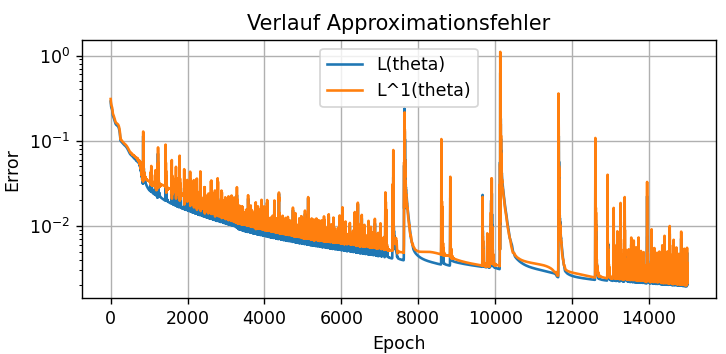
\includegraphics[width=0.7\textwidth]{papers/neuronal/images/approximation_error_burgers.png}
    \caption{Verlauf des Approximationsfehlers der Burgers-Gleichung}
    \label{fig:fehler_burgers}
\end{figure}

Wertet man das neuronale Netzwerk über die Bereiche von \( x \) und \( t \) aus, ergibt sich ein Plot der Lösung des neuronalen Netzwerks (siehe Abbildung \ref{fig:loesung_burgers}).
\begin{figure}
    \centering
    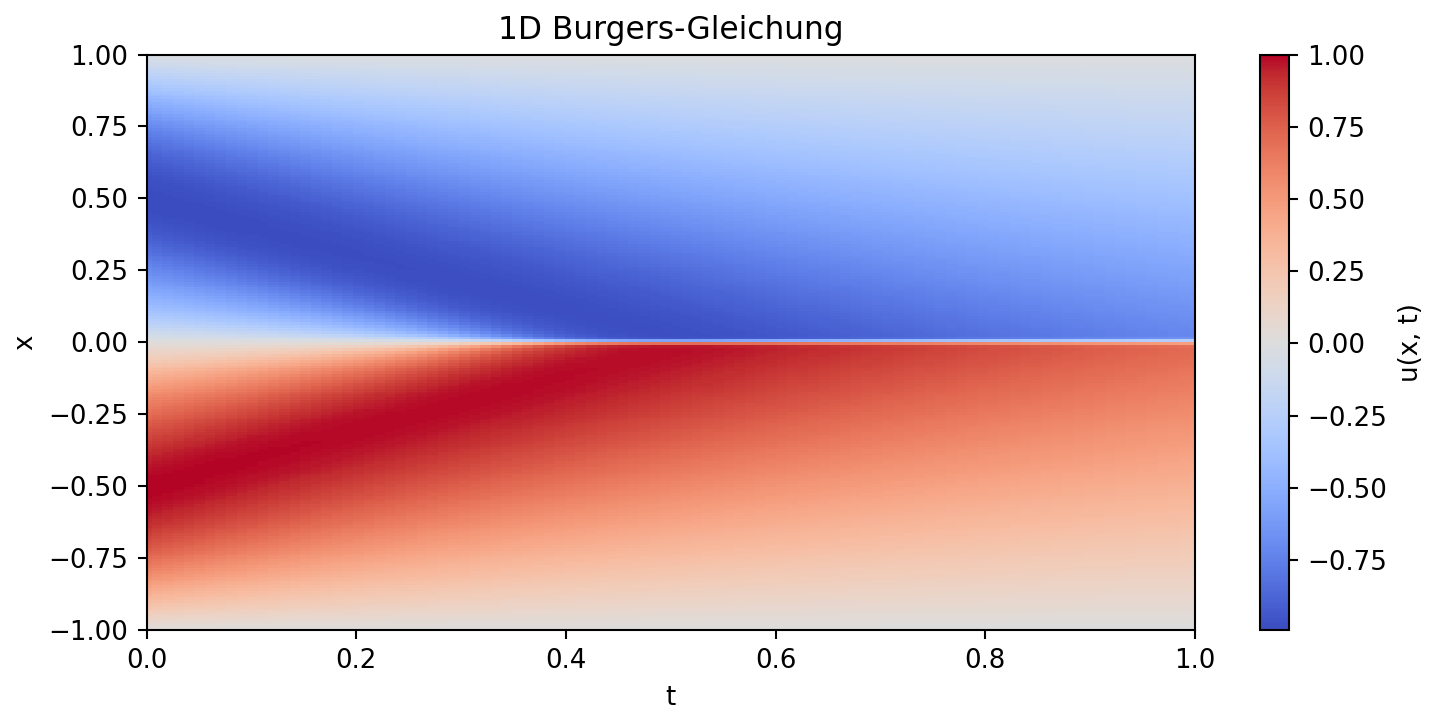
\includegraphics[width=0.8\textwidth]{papers/neuronal/images/prediction_burgers_net.png}
    \caption{Lösungs-Plot der Burgers-Gleichung}
    \label{fig:loesung_burgers}
\end{figure}

Der gesamte Code zur Umsetzung ist im GitHub-Repository des Seminars abgelegt \cite{neuronal:github_source_code}.

